\documentclass[Main]{subfiles}
\begin{document}

\chapter{Java Remote Method Invocation}
This chapter will cover the fundamentals in Java Remote Method Invocation (RMI) and how a leader of the collaboration is elected.

\section{JAVA RMI}
Java Remote Method Invocation (RMI) is a middleware that supports Java-to-Java only. RMI gives a client on one Java Virtual Machine (JVM) access to objects that runs on another JMV which allows the client to invoke methods on the object - called the Remote Object \cite{RMI-slides}. A JVM is a virtual machine that executes an application written in Java bytecode \cite{wiki-jvm}.

\begin{figure}[H]
\centering
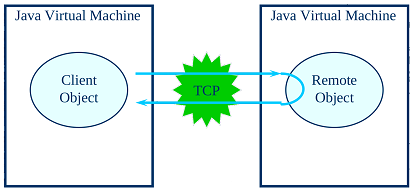
\includegraphics[scale=1]{Figurer/JVM.png}
\caption{A simple Java API containing two JVM's \cite{RMI-slides}}
\end{figure}


\section{Leader election}



\end{document}  